\section{\sysname{} Design}

We design the \sysmodlong{} (\sysmod{}) based on the definitions in
previous section.
A \sysmod{} represents a single distributed system with specific semantics
and \sysname{} can perform individual \sysmod{} validation to check if all
semantic constraints are sound and compatible, as
well as pairwise checks between two \sysmods{} to determine if one
is satisfiable under another's constraints.
More importantly, \sysname{} can model applications that rely on multiple
distributed systems with different
consistency semantics (i.e., \sysmods{}) and can check for compatibility
between the application logic and the assigned semantics by performing a
compositional check using the \sysgraph{}.

\subsection{Compatibility Check}

\sysname{} is designed to reason about
compatibility among consistency semantics.
We define compatibility between two consistency semantics using \sysmods{}
$M_1$ and $M_2$ using
an implication-based criterion. $M_1$ is considered compatible with
$M_2$ if the formula $M_1 \Rightarrow M_2$ is valid, i.e., there is no
execution that satisfies all constraints of $M_1$ without also
satisfying $M_2$.
We implement this by asserting the negation $\neg (M_1 \Rightarrow M_2)$ and
checking if it is unsatisfiable using our SMT-based approach. If no
counterexample can be found, it implies that $M_1$
refines/subsumes $M_2$. This compatibility check is not symmetric:
$M_1 \Rightarrow M_2$
holding does not necessarily mean that $M_2 \Rightarrow M_1$ also holds.

Table \ref{tab:pairwise-time} shows a result of pairwise
compatibility checks for
base semantics in \sysname{} which in part shows that our consistency
models' compatibility faithfully matches with the theoretical results
in \cref{fig:semantics-tree} and in previous literature \cite{terry1994session}.

To combine multiple consistency models into a single stronger model, we used
logical conjunctions on each \sysmod{}'s constraints. By taking the constraints
representing each model's semantics and forming their conjunction, we derive a
composed model that enforces all included constraints simultaneously.
This approach allows incremental composition: users can start from a
base model and iteratively strengthen it by adding new sets of constraints,
either from our implemented models or user-defined constraints, representing
additional consistency guarantees.

\subsection{\sysgraph{} and Composition Check}
\label{subsec:search}
%. Components (e.g., functionality)
%of an application are modeled as nodes and data flow and constraints
%between systems are represented as edges connecting the nodes in the
%\sysgraph{}. \sysname{} can check specific assignments of distributed
%system semantics or outputs results of all satisfiable assignments
%for the \sysgraph{}.

\usetikzlibrary{arrows.meta, positioning, calc, fit}

% Preamble (once):
% \usetikzlibrary{arrows.meta, positioning, calc, fit}

% Preamble (once):
% \usetikzlibrary{arrows.meta, positioning, calc, fit}

\begin{figure}[t]
\centering
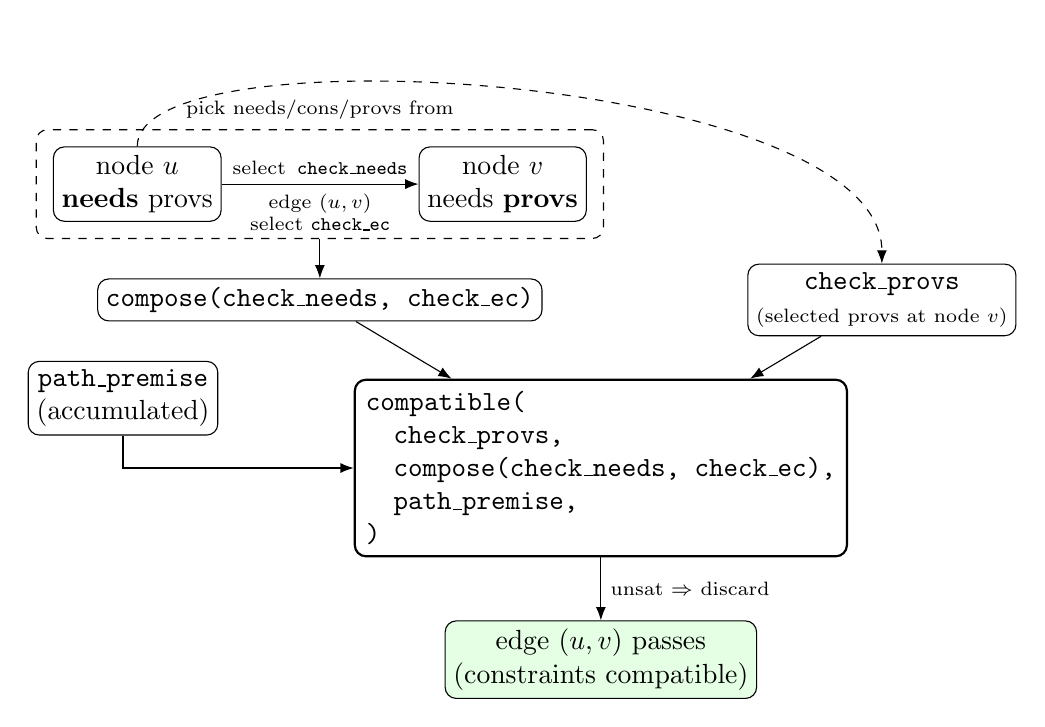
\begin{tikzpicture}[
  node distance=12mm,
  box/.style={draw, rounded corners, align=center, inner sep=3pt},
  boxwide/.style={draw, rounded corners, align=left, inner sep=4pt},
  lbl/.style={font=\scriptsize},
  ->, >=Latex
]
% nodes
\node[box] (u) {node $u$ \\ \textbf{needs} provs};
\node[box, right=25mm of u] (v) {node $v$ \\ needs \textbf{provs}};
% group box
\node[draw, dashed, rounded corners, fit=(u)(v), inner sep=6pt,
      label=above:{\scriptsize pick needs/cons/provs from \sysgraph}] (sel) {};
% compose
\node[box] (compose) [below=5mm of sel] {\texttt{compose(check\_needs, check\_ec)}};
% premise
\node[box] (path) [below=5mm of compose, xshift=-25mm] {$\texttt{path\_premise}$ \\ (accumulated)};
% provs
\node[box] (provs) [right=26mm of compose] {$\texttt{check\_provs}$ \\ {\scriptsize (selected provs at node $v$)}};

% compat
\node[boxwide, thick] (compat) [below=10mm of $(compose)!0.5!(provs)$] {%
\texttt{compatible(}\\
\quad \texttt{check\_provs,}\\
\quad \texttt{compose(check\_needs, check\_ec),}\\
\quad \texttt{path\_premise,}\\
\texttt{)}};

% result
\node[box, fill=green!10] (ok) [below=8mm of compat] {edge $(u,v)$ passes \\ (constraints compatible)};

% arrows
\draw[->]
  (u) -- node[lbl, above] {select $\,\texttt{check\_needs}$}
        node[lbl, below, align=center] {edge $(u,v)$\\select $\texttt{check\_ec}$} (v);
\draw[->, dashed] (u.north) .. controls +(0,15mm) and +(0,24mm) .. (provs.north);
\draw[->] (sel.south) -- (compose);
\draw[->] (compose) -- (compat);
\draw[->] (provs) -- (compat);
\draw[->] (path) |- (compat);
\draw[->] (compat) -- node[lbl, right] {unsat $\Rightarrow$ discard} (ok);
\end{tikzpicture}
\caption{Example flow for a single edge $(u,v)$: choose a tuple of \texttt{needs} (node $u$), \texttt{cons} (edge $(u,v)$), and \texttt{provs} (node $v$); compute \texttt{compose(needs, cons)}; check \texttt{compatible} against \texttt{provs} under the accumulated \texttt{path\_premise}. For multigraphs, repeat this per parallel edge (or combination of multiple edges) with its own chosen \texttt{cons} tuple.}
\label{fig:skel}
\end{figure}

Applications that rely on multiple distributed systems with different
consistency semantics can be checked for correctness by performing a
compositional check using the \sysgraph{}.
Our composability check
verifies if a distributed application, modeled as a graph (\ie
\sysgraph{}) can have its components interact in a way that
respects their individual consistency requirements and guarantees.

%The function checks if there exists at least one valid way to assign
%specific semantics (from the choices provided in needs/provs/cons)
%such that all interactions are consistent.

% The \sysgraph{} is composed of \textit{nodes} with two fields:
% (1) \textit{needs}, required constraint tuples from dependent components, and
% (2) \textit{provs}, constraint tuples it provides to other nodes.
% \sysname{} users can freely specify application logics, and each node
% has both \textit{needs} and \textit{provs}, with either our predefined built-in
% \sysmods{} or user-defined
% constraints that represent the node's semantics using our interface.
% \textit{Edges} connect nodes and have the \textit{cons} field,
% specific constraint tuples for the node pair interaction.
% In pluggable constraints for \textit{needs}, \textit{provs}, and \textit{cons},
% users may use (1) pre-build or bring-your-own \sysmods representing consistency semantics,
% (2) application-level and application-specific logic.
% The tuples within the list represent constraints that must hold together
% (logical \textsc{and}).

The \sysgraph{} is composed of \textit{nodes} with two fields:
(1) \textit{needs}, required constraint tuples from dependent components, and
(2) \textit{provs}, constraint tuples provided to other nodes.
Each node's semantics can be expressed using our predefined consistency \sysmods{}
or user-defined constraints that implement the same interface. Edges connect nodes
and carry \textit{cons}, constraint tuples for that node pair's interaction.
Each tuple is a conjunction of constraints.

For pluggable constraints in \textit{needs}, \textit{provs}, and \textit{cons},
users can combine:
(1) consistency semantics (pre-built or custom \sysmods{}), and
(2) application-level or application-specific logic.

In the implementation (also see Fig. \ref{fig:skel}), we perform a depth-first search (DFS) starting from a
given source node, keeping track of visited edges and the accumulated
constraints in \texttt{path\_premise}, along the current path.
\sysname{} performs compatibility checks, \texttt{compatible(check\_provs,
compose(check\_needs, check\_ec), path\_premise)}:
for each edge $(u, v)$ from the current node $u$, it checks if \texttt{provs} from $v$
and \texttt{cons} from edge $(u, v)$ satisfy needs from $u$.
This checks if the chosen path provides guarantee of the destination
(\texttt{check\_provs}) is
implied by the conjunction (the result returned from call to \texttt{compose}) of the chosen needs of the
source (\texttt{check\_needs}) and the chosen edge constraints
(\texttt{check\_ec}),
considering the constraints already accumulated (\texttt{path\_premise}).

If all checks succeed then the application is proven to be compatible
with the plugged-in \sysmods{} and the application logics are also
sound as a whole.

\subsection{Compatible Combination Search}

\sysname{} is capable of searching for compatible \sysmods{} for an
application given an \sysgraph{}. When blank \sysmods{} are plugged into the
\sysgraph{}, \sysname{} searches for compatible combinations of
\sysmods{} for the user.
Considering that strictly weaker distributed semantics can be replaced
with strictly stronger ones and the weaker semantics are typically
more performant and cheaper to maintain, \sysname{} searches the space
in an order that prioritizes weaker semantics. Specifically, we give scores
0 to 5 to semantics in the columns from left to right in
\cref{fig:semantics-tree}
and test the combination that has lower sum of scores first during the search.
If compatible combinations are found, the search can stop early; replacing a
\sysmod{} in a compatible combination with a strictly stronger one is always
guaranteed to be compatible.
However, our search strategy is not optimal and investigating more
efficient search algorithms remains as future work.

%If a compatible combination is found that satisfies all unvisited edges
%between u and v at the current step, it adds the chosen constraints
%(needs, provs, cons) to the result graph, updates the path\_premise
%by composing the newly satisfied constraints, marks the edges as
%visited, and continues the DFS from the destination node v. If the
%DFS eventually visits all edges in the graph, the function returns
%True and the result graph showing one valid assignment. If a dead end
%is reached or no compatible combination works for an edge, it
%backtracks, removing the choices made at that step and trying other
%combinations. If the DFS completes without visiting all edges
%(meaning no fully consistent assignment was found), it returns False.

%% TODO: can be better
%After a successful composable check, our extraction function
%(\texttt{extract(inode, onode, result)}) takes the resulting graph
%from composability check (which represents one valid assignment of
%constraints) and aggregates a single Z3 constraint that
%represents the net or equivalent semantic guarantee of the subgraph
%reachable from a specific node (inode), assuming inode and onode are
%the same. The function performs a DFS (dfs helper) starting from the
%specified inode on this result graph. For each edge (src, dst)
%traversed in the DFS, the extraction function uses the specific provs
%constraint assigned to src in the result graph, uses the specific
%needs constraint assigned to dst in the result graph, and retrieves
%the specific cons constraint assigned to the edge (src, dst, k) in
%the result graph. The extract function creates a composite constraint
%for this single edge interaction: compose(src\_provs, edge\_cons,
%dst\_needs). This represents the conjunction of constraints relevant
%to this specific step in the flow. It collects these composite
%constraints from all edges reachable from inode in the DFS. Finally,
%it returns the logical \textsc{and} (compose) of all collected composite
%constraints. Simply put, axioms and relations define constraints on
%Operations; similarly, extract defines a summary constraint on a
%successfully composed subgraph. If the composable check found a valid
%way for components A, B, and C to interact starting from A,
%extract(A, A, result) generates a single formula representing the
%overall guarantee provided by the A→B→C... chain, as seen from A's
%perspective, based on the specific choices made during the composability check.
%
%
